\newpage
\section{Using the Integrator}
\genHeader
\label{sec:app_integrator}

% New interface? When reach this point, user will have a working TGG with 3 partitions, 3 entires. Explain the process via integrator

Let's check out another visualization feature of eMolfon, the integrator! While the graph view `see' the construction and result of the triple
metamodel \texttt{.xmi} files, the integrator enables you to trace each of these created in the transformation process. The integrator works as an ``offline''
debugger, working on the protocol (trace) of the transformation.

\begin{itemize}

\item[$\blacktriangleright$] Right-click on \texttt{corr\_BWD.xmi} and choose ``eMoflon $\rightarrow$ Start Integrator'' which will open the window depicted in
Fig.~\ref{fig:integrator_start}.

\begin{figure}[htbp]
\begin{center}
  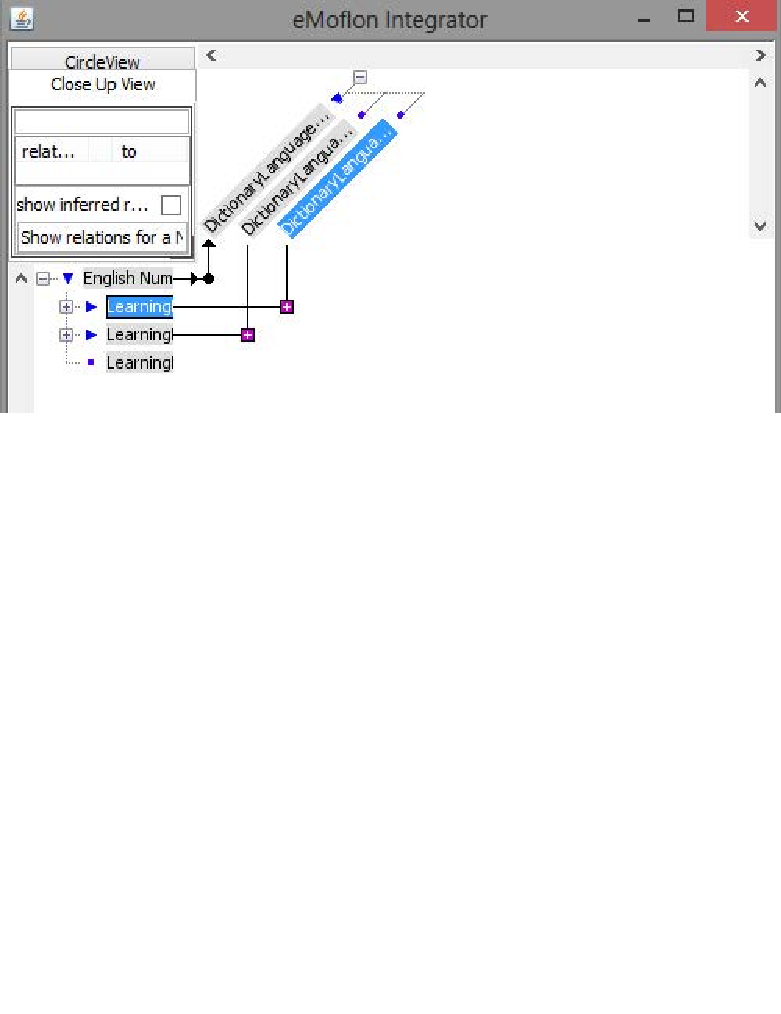
\includegraphics[width=0.7\textwidth]{integrator_start_view.pdf}
  \caption{Default view of the integrator}
  \label{fig:integrator_start}
\end{center}
\end{figure}

\item[$\blacktriangleright$] Drag and drop \texttt{protocol\_BWD.xmi} into the main window.\footnote{If the integrator window minimizes, press \texttt{alt+tab}
to re-activate it} You will now see the navigation controls explained in the lower part of the window (Fig.~\ref{fig:integrator_after_protocol}).

\begin{figure}[h!]
\begin{center}
  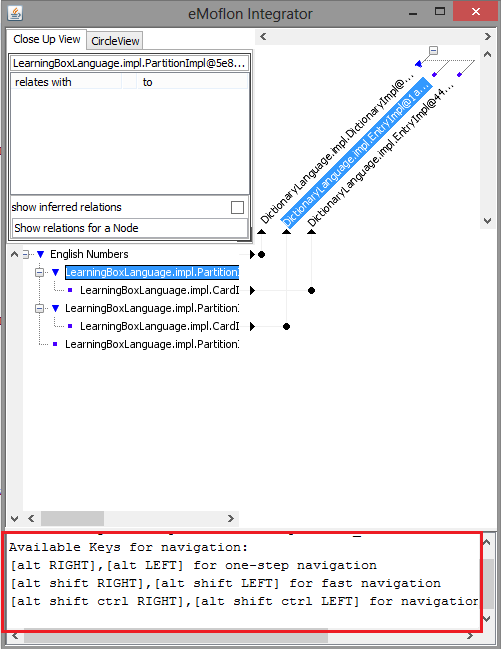
\includegraphics[width=0.6\textwidth]{integrator_after_protocol_insertion.png}
  \caption{Integrator after protocol insertion.}
  \label{fig:integrator_after_protocol}
\end{center}
\end{figure} 

\item[$\blacktriangleright$]  Starting at \texttt{Box}, you can use \texttt{Alt+Right} to navigate forwards \emph{through} the transformation process, and
\texttt{Alt+Left} to go backwards -- each step will appear in the smaller window below!

\item[$\blacktriangleright$] It lists which element it is currently working with, and then checks \emph{every} possible rule that could be applied. I.e.,
suppose we had two or three different \texttt{BoxToDictionary} rules, all defined slightly differently. What the TGG does, and the integrator displays, is how
each \texttt{card} is checked for each one of those rules. Even if the first rule is checked first and found applicable, it will \emph{still} check the other
two rules before moving on. If two rules are able to be applied, you will be prompted to choose.

\newpage

\item[$\blacktriangleright$] While you're stepping through the transformation, you will notice that some elements are highlighted with colours. These are the
elements currently being processed, and the colours have the following definitions:

\begin{description}
  \item[Blue] The element is now about to be processed (is being ``looked at'').
  
  \item[Yellow] The element cannot be transformed right now and has been queued for later transformation (i.e., when transforming an Entry to a Card, the Box
  with partitions to put the Card into must be translated first).
  
  \item[Green] The object has been created.
\end{description}

End Text.

\end{itemize}
